\documentclass[a4paper,11pt]{book}
%\documentclass[a4paper,twoside,11pt,titlepage]{book}
\usepackage{listings}
\usepackage[utf8]{inputenc}
\usepackage[spanish]{babel}

% \usepackage[style=list, number=none]{glossary} %
%\usepackage{titlesec}
%\usepackage{pailatino}

%\decimalpoint
\usepackage{dcolumn}
\usepackage{float}
\newcolumntype{.}{D{.}{\esperiod}{-1}}
\makeatletter
%\addto\shorthandsspanish{\let\esperiod\es@period@code}
\makeatother


%\usepackage[chapter]{algorithm}
\RequirePackage{verbatim}
%\RequirePackage[Glenn]{fncychap}
\usepackage{fancyhdr}
\usepackage{graphicx}
\usepackage{afterpage}

\usepackage{longtable}

\usepackage[pdfborder={000}]{hyperref} %referencia

% ********************************************************************
% Re-usable information
% ********************************************************************
\newcommand{\myTitle}{Trabajo 2 - Evaluación Continua\xspace}
\newcommand{\myDegree}{MÁSTER EN INVESTIGACIÓN EN INGENIERÍA DE SOFTWARE Y
SISTEMAS INFORMÁTICOS\xspace}
\newcommand{\myName}{César Hugo Bárzano Cruz\xspace}
\newcommand{\myProf}{Nombre Apllido1 Apellido2 (tutor1)\xspace}
\newcommand{\myOtherProf}{Nombre Apllido1 Apellido2 (tutor2)\xspace}
%\newcommand{\mySupervisor}{Put name here\xspace}
\newcommand{\myFaculty}{ Universidad Nacional de Educación a Distancia\xspace}
\newcommand{\myFacultyShort}{UNED-Facultad de informática\xspace}
\newcommand{\myDepartment}{\xspace}
\newcommand{\myUni}{\protect{ Universidad Nacional de Educación a Distancia}\xspace}
\newcommand{\myLocation}{Madrid\xspace}
\newcommand{\myTime}{\today\xspace}
\newcommand{\myVersion}{Version 0.1\xspace}


\hypersetup{
pdfauthor = {\myName hugobarzano@gmail.com},
pdftitle = {\myTitle},
pdfsubject = {},
pdfkeywords = {},
pdfcreator = {LaTeX con el paquete TEXmaker},
pdfproducer = {pdflatex}
}

%\hyphenation{}


%\usepackage{doxygen/doxygen}
%\usepackage{pdfpages}
\usepackage{url}
\usepackage{colortbl,longtable}
\usepackage[stable]{footmisc}
%\usepackage{index}

%\makeindex
%\usepackage[style=long, cols=2,border=plain,toc=true,number=none]{glossary}
% \makeglossary

% Definición de comandos que me son tiles:
%\renewcommand{\indexname}{Índice alfabético}
%\renewcommand{\glossaryname}{Glosario}

\pagestyle{fancy}
\fancyhf{}
\fancyhead[LO]{\leftmark}
\fancyhead[RE]{\rightmark}
\fancyhead[RO,LE]{\textbf{\thepage}}
\renewcommand{\chaptermark}[1]{\markboth{\textbf{#1}}{}}
\renewcommand{\sectionmark}[1]{\markright{\textbf{\thesection. #1}}}

\setlength{\headheight}{1.5\headheight}

\newcommand{\HRule}{\rule{\linewidth}{0.5mm}}
%Definimos los tipos teorema, ejemplo y definición podremos usar estos tipos
%simplemente poniendo \begin{teorema} \end{teorema} ...
\newtheorem{teorema}{Teorema}[chapter]
\newtheorem{ejemplo}{Ejemplo}[chapter]
\newtheorem{definicion}{Definición}[chapter]

\definecolor{gray97}{gray}{.97}
\definecolor{gray75}{gray}{.75}
\definecolor{gray45}{gray}{.45}
\definecolor{gray30}{gray}{.94}

\lstset{ frame=Ltb,
     framerule=0.5pt,
     aboveskip=0.5cm,
     framextopmargin=3pt,
     framexbottommargin=3pt,
     framexleftmargin=0.1cm,
     framesep=0pt,
     rulesep=.4pt,
     backgroundcolor=\color{gray97},
     rulesepcolor=\color{black},
     %
     stringstyle=\ttfamily,
     showstringspaces = false,
     basicstyle=\scriptsize\ttfamily,
     commentstyle=\color{gray45},
     keywordstyle=\bfseries,
     %
     numbers=left,
     numbersep=6pt,
     numberstyle=\tiny,
     numberfirstline = false,
     breaklines=true,
   }

% minimizar fragmentado de listados
\lstnewenvironment{listing}[1][]
   {\lstset{#1}\pagebreak[0]}{\pagebreak[0]}

\lstdefinestyle{CodigoC}
   {
	basicstyle=\scriptsize,
	frame=single,
	language=C,
	numbers=left
   }
\lstdefinestyle{CodigoC++}
   {
	basicstyle=\small,
	frame=single,
	backgroundcolor=\color{gray30},
	language=C++,
	numbers=left
   }


\lstdefinestyle{Consola}
   {basicstyle=\scriptsize\bf\ttfamily,
    backgroundcolor=\color{gray30},
    frame=single,
    numbers=none
   }


\newcommand{\bigrule}{\titlerule[0.5mm]}


%Para conseguir que en las páginas en blanco no ponga cabecerass
\makeatletter
\def\clearpage{%
  \ifvmode
    \ifnum \@dbltopnum =\m@ne
      \ifdim \pagetotal <\topskip
        \hbox{}
      \fi
    \fi
  \fi
  \newpage
  \thispagestyle{empty}
  \write\m@ne{}
  \vbox{}
  \penalty -\@Mi
}
\makeatother

\usepackage{pdfpages}
\begin{document}
\begin{titlepage}
 
 
\newlength{\centeroffset}
\setlength{\centeroffset}{-0.5\oddsidemargin}
\addtolength{\centeroffset}{0.5\evensidemargin}
\thispagestyle{empty}

\noindent\hspace*{\centeroffset}\begin{minipage}{\textwidth}

\centering

\includegraphics[width=0.7\textwidth]{imagenes/Logo-uned.jpg}\\[1.1cm]


{\Huge\bfseries Máster Universitario En Investigación En Ingeniería De Software Y Sistemas Informáticos\\
}
\noindent\rule[-1ex]{\textwidth}{3pt}\\[3.5ex]
{\large\bfseries Generación Automática de Código}
\end{minipage}

\vspace{2.5cm}
\noindent\hspace*{\centeroffset}\begin{minipage}{\textwidth}
\centering

\textbf{Autor}\\ {César Hugo Bárzano Cruz}\\[2.5ex]


\includegraphics[width=0.3\textwidth]{imagenes/Logo-master.png}\\[0.1cm]
\textsc{Trabajo 1 De Evaluación Continua}\\
\textsc{---}\\
2017/2018
\end{minipage}
%\addtolength{\textwidth}{\centeroffset}
%\vspace{\stretch{2}}
\end{titlepage}




%\frontmatter
\tableofcontents
\listoffigures
%\listoftables

%
%\mainmatter
%\setlength{\parskip}{5pt}

%\input{capitulos/01_Introduccion}


\chapter{Introducción}

El presente documento representa la memoria formal para evaluación continua de la segunda práctica de la asignatura  Generación Automática de Código. Dicha práctica consiste en un generador de datos en formatos (CSV , HTML , XML, JSON) como salida a partir de un sistema de gestion de bases de datos (SGBD) relacional como entrada.  

En los siguientes capítulos se detallará la solución propuesta, las tecnologías utilizadas, se analizarán las ventajas e inconvenientes de la solución propuesta, se explicarán los casos de uso o pruebas a los que se ha sometido el generador, se explicará como utilizar correctamente el generador así como las dependencias necesarias para su correcto uso. 

Finalmente se analizarán las tareas y conocimientos adquiridos en esta práctica junto con un anexo de los documentos necesarios.   



\chapter{Desarrollo de la Práctica}

\section{Tecnologías Utilizadas}

Como tecnología base, se ha decidido utilizar el lenguaje de programación interpretado Python\cite{py}, versión 2.7.15 debido a la sencillez y capacidad del mismo para proporcionar una solución. 

Como se indicó en la introducción, la entrada del generador a impletar es uno o varios sistemas de gestión de bases de datos(SGBD). Los SGBDs que este generador soporta son los siguientes:

\begin{enumerate}
\item \textbf{mysql}
\item \textbf{postgres}
\item \textbf{sqlite3}
\end{enumerate}
 
El sistema operativo base sobre el que se han realizado las pruebas es Ubuntu 18.04 LTS

Adicionalmente para la confección de esta memoria se ha utilizado LaTEX con el paquete de librerías texlive-full y el editor texmaker. Los siguientes enlaces muestran como instalar y utilizar correctamente LaTEX, han sido utilizados como referencia para el presente documento. 

\begin{enumerate}
\item \href{http://milq.github.io/install-latex-ubuntu-debian/}{Instalar LaTeX}
\item \href{ http://minisconlatex.blogspot.com.es/}{Usar LaTeX}
\end{enumerate}
 
\section{Especificación de la Solución}

Las posibles especificaciones e implementaciones para un generador como el propuesto por el enunciado pueden ser muy variadas. Dichas especificaciones pueden variar significativamente en función de las tecnologías utilizadas, las aserciones o comprobaciones de robustez que se quieran realizar a las entradas, al procesamiento o a las salidas, los posibles casos que se quieran tener en cuenta así como el grado de modularidad que se quiera alcanzar de cara a futuras actualizaciones.

El generador utiliza a modo de configuración un fichero Json en el que vienen especificados los parametros necesarios para establecer la conexión con los distintos SGBD soportados. Un Ejemplo de entrada para este fichero de configuración es el siguiente: 

\begin{lstlisting}[language=python,caption={ Entrada Unitaria Configuración Generador }]
{
...

"mysql_1": {
		"user": "user",
		"password": "pass",
		"host": "host",
		"database": "database"
	},
...
}
\end{lstlisting}

Las entradas usan como clave el identificador del tipo de SGBD, esto permite al generador diferenciar el tipo de conector a usar para poder extraer los datos, es decir, mysql\_n establece la informacion necesaria para conectarse al SGBD número N basado en mysql. Esto permite configurar tantos SGBD basados en mysql como se quiera. El siguiente ejemplo muestra un ejemplo de configuración más completo en el que se incluyen todos los SGBD soportados por el generador: 

\begin{lstlisting}[language=python,caption={ Entrada Completa Configuración Generador }]

{
 	"mysql_1": {
 		"user": "user",
 		"password": "pass",
 		"host": "host",
 		"database": "database"
 	},
 	"mysql_2": {
 		"user": "user2",
 		"password": "pass2",
 		"host": "host2",
 		"database": "database2"
 	},
 	"postgres_1": {
 		"user": "postgres",
 		"password": "123456",
 		"host": "host",
 		"database": "database"
 	},
 	"sqlite3_1": {
 		"db_path": "path/to/database/file"
 	}
 }
\end{lstlisting}

Como podemos observar en el ejemplo anterior, el fichero de configuración para el generador nos permite definer tantos SGBD como necesitemos inidcando siempre el indicador de tecnología: mysql\_N, postgres\_N o sqlite3\_N.

En los casos de mysql y postgres es necesario establecer la configuración necesaria para la conexión indicando usuario, contraseña, host (url o ip) y base de datos a la que conectar. De manera adicional el genrador soporta sqlite3 pero debido a ser esta una base de datos para pruebas generalmente en local, la información necesaria es el path al fichero en disco que actua como base de datos. Para este último caso es necesario tener en cuenta que dicho fichero tiene que tener los permisos adecuados (lectura almenos) para que el generador sea capaz de leer la información de dicha base de datos. 


El generador cuenta con la siguiente ayuda con el objetivo de facilitar la comprensión de los argumentos que necesita para un uso nominal. 


\begin{lstlisting}[language=python,caption={ python generadorP2.py --help }]

Usage: python generador.py [options]

Options
-v, --version			Show the version of this script
-h, --help			Show this help.
-t <table_name>, --table <table_name>   Input database table
-w <"column = 'value'">, --where <"column = 'value'">   Optional Where Clause
-d,         --debug         	Debug Mode

\end{lstlisting}

Como podemos observar en la ayuda del generador, es necesario el flag -t o --table para indicar la tabla de la cual el generador va a extraer la información  dentro de los distintos SGBD establecidos en la configuración. 

De manera adicional, se puede añadir el flag -w o --where para filtar utilizando la clausula relacional WHERE. 

Con el objetivo de facilitar la comprensión de que hace el generador en cada etapa de su ejecución, se ha incluido el flag -d o --debug el cual permite ver por la salida estándar que acción esta realizando el generador.   

Tras una ejecución, el generador creará en el directorio OUTPUT 4 ficheros por cada uno de los SGBD especificados con la siguiente convención de nombres:

\begin{enumerate}
\item \textbf{GAC\_mysql\_1\_20180820\_203859.csv}
\item \textbf{GAC\_mysql\_1\_20180820\_203859.html}
\item \textbf{GAC\_mysql\_1\_20180820\_203859.json}
\item \textbf{GAC\_mysql\_1\_20180820\_203859.xml}
\end{enumerate}

\section{Análisis de la solución}

	Se considera que la solución propuesta es valida, ya que cumple con lo solicitado, realiza las adecuadas comprobaciones para una correcta ejecución, genera los distintos formatos esperados y además se ha alcanzado de una manera sencilla, en un solo script python junto con los conectores necesarios para cada uno de los SGBD tratados. La modularidad de la solución propuesta favorece posibles actualizaciones del generador, incluyendo en el bucle de iteración principal el conector necesario para soportar nuevas bases de datos. El generador carga su configuración mediante variables de entorno ( GENERATOR\_CONFIG ) lo que permite cambiar rapidamente el tipo de configuración a utilizar en cada ejecución. 

La solución alcanzada no es completa debido a los conectores con las bases de datos, ya que como se ha explicado antes solo soporta 3 SGBD por lo que quizas esta seria su principal defecto. 
 
\section{Pruebas}

Con el Objetivo de mostrar la potencia del generador, se van a realizar una serie de ejecuciones de prueba para mostrar todos los posibles escenarios del generador. Para ello es necesario disponer de los 3 tipos de SGBD soportadas por el generador con datos significaticos que exportar. Para ello se incluye el fichero init.py cuyo objetivo es el de añadir entradas a las bases de datos instaladas localmente en mi equipo. 

Para facilitar los distintos escenarios de pruebas a los que vamos a someter al generador, se va a utlizar el usuario root con password root para la base de datos mysql , una base datos postegres cuyo usuario y contraseña es postgres:123456 y como detallamos anteriormente una base de datos sqlite3 representada por un fichero en disco.


Adicionalmente se va a mostrar ciertos casos de error tenidos en cuenta en la implementación de la solución, por lo que se propone dividir esta sección en las siguientes sub-secciones. Para automatizar este proceso se ha creado el Makefile que se adjunta en al anexo donde se especifica cada uno de los testCases\_N.sh que serán ejecutados, tomando como entrada los ficheros alojados en el directorio input y dejando el resultado en el directorio output. En las capturas que muestran cada una de las pruebas se ve todo lo necesario para su ejecución.  

\subsection{Pruebas de Funcionalidad}
Para mostrar la correcta funcionalidad del generador se va a comenzar exportando datos de cada uno de los SGBD de manera independiente. Tras esto, se ejemplificará el uso de la clausula WHERE para filtrar los datos a exportar y finalmente se mostrarán casos de pruebas mas complejos en los que se atará con una sola ejecuación a todos los SGBD soportados por el generador.  

\subsubsection{Test Case 1 - mysql}

A continuación se muestra la configuración utilziada por el generador para el primer caso de pruaba. 

\begin{lstlisting}[language=python,caption={GAC\_GENERATOR\_CONFIG\_1.json }]
 {
	"mysql_1": {
		"user": "root",
		"password": "root",
		"host": "localhost",
		"database": "testGAC"
	}
}
\end{lstlisting}

Utilizando la linea de ordenes para mysql, podemos observar cual es el estado interno del SGBD

\begin{figure}[H]  
\centering 
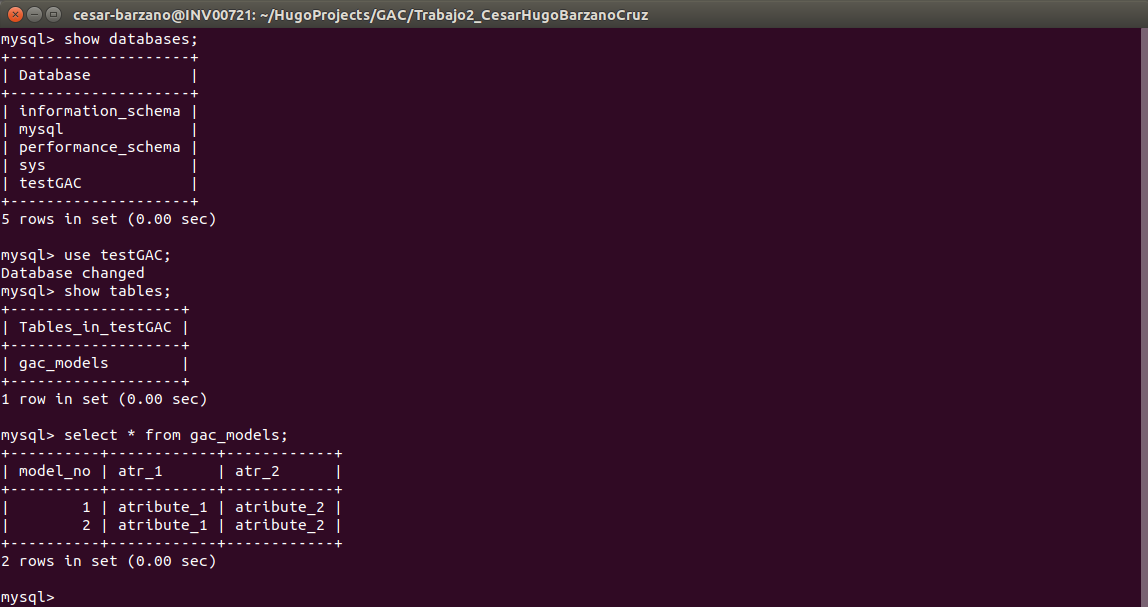
\includegraphics[scale=0.35]{imagenes/TestCase1_mysql.png}
\caption{ Mysql status  }  
\end{figure} 

Ejecutando el primer caso de prueba mediante make testCase1, el generador mostrará por pantalla lo siguiente: 

\begin{figure}[H]  
\centering 
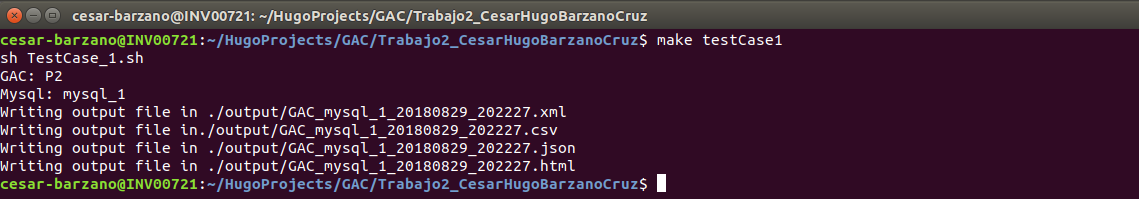
\includegraphics[scale=0.35]{imagenes/TestCase1_1.png}
\caption{ Test Case 1  }  
\end{figure} 

La ejecución del primer caso de prueba produce las siguientes salidas dentro del directorio output


\begin{lstlisting}[language=python,caption={Formato CSV }]
1,atribute_1,atribute_2
2,atribute_1,atribute_2
\end{lstlisting}

\begin{lstlisting}[language=python,caption={Formato HTML }]
<!DOCTYPE html>
    <html>
    <head>
    <title>mysql_1</title>
    </head>
    <body>
    <h1>mysql_1</h1><hr><br><table style="width:100%"><tr><td>2</td><td>atribute_1</td><td>atribute_2</td></tr></table></body></html> 
\end{lstlisting}

El resultado del generador para formato HTML queda mas claro si es interpretado por el navegador: 

\begin{figure}[H]  
\centering 
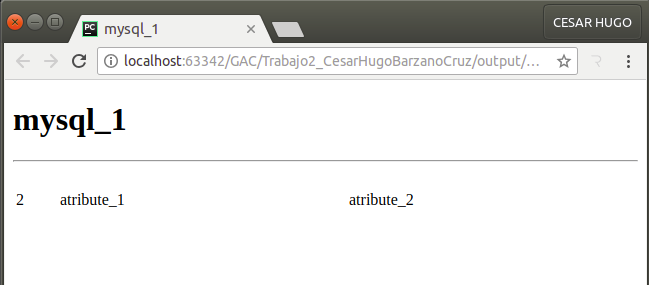
\includegraphics[scale=0.35]{imagenes/TestCase1_html.png}
\caption{ Test Case 1 - HTML Output }  
\end{figure} 


\begin{lstlisting}[language=python,caption={Formato Json }]
[[1, "atribute_1", "atribute_2"], [2, "atribute_1", "atribute_2"]]
\end{lstlisting}


\begin{lstlisting}[language=python,caption={Formato XML }]
<data>&lt;data&gt;&lt;i&gt;&lt;i&gt;1&lt;/i&gt;&lt;i&gt;atribute_1&lt;/i&gt;&lt;i&gt;atribute_2&lt;/i&gt;&lt;/i&gt;&lt;i&gt;&lt;i&gt;2&lt;/i&gt;&lt;i&gt;atribute_1&lt;/i&gt;&lt;i&gt;atribute_2&lt;/i&gt;&lt;/i&gt;&lt;/data&gt;</data>
\end{lstlisting}

El resultado del generador para formato xml queda mas claro si es interpretado por el navegador: 

\begin{figure}[H]  
\centering 
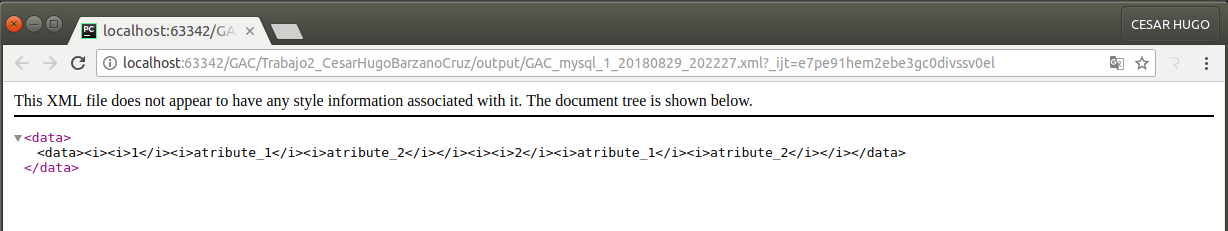
\includegraphics[scale=0.35]{imagenes/TestCase1_xml.png}
\caption{ Test Case 1 - XML Output }  
\end{figure} 

\subsubsection{Test Case 2 - Postgres}

A continuación se muestra la configuración utilizada por el generador para el segundo caso de pruaba. 

\begin{lstlisting}[language=python,caption={GAC\_GENERATOR\_CONFIG\_2.json }]
 {
  "postgres_1": {
		"user": "postgres",
		"password": "123456",
		"host": "127.0.0.1",
		"database": "testgac"
  }
}
\end{lstlisting}

Utilizando la linea de ordenes para Postgres, podemos observar cual es el estado interno del SGBD. Por simplicidad la estructura de la base de datos es similiar a mysql. 

\begin{figure}[H]  
\centering 
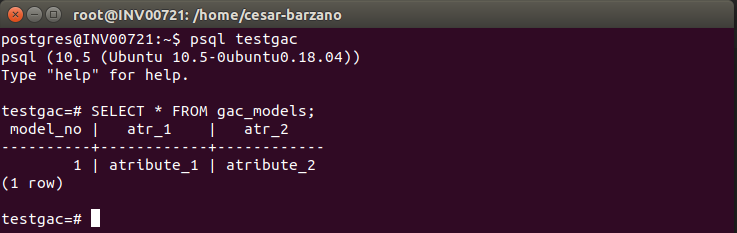
\includegraphics[scale=0.35]{imagenes/TestCase2_postgres.png}
\caption{ Postgres status }  
\end{figure} 

El segundo caso de prueba puede ejecutarse mediante make testCase2, el resultado es similitar al caso de prueba 1. 

\begin{figure}[H]  
\centering 
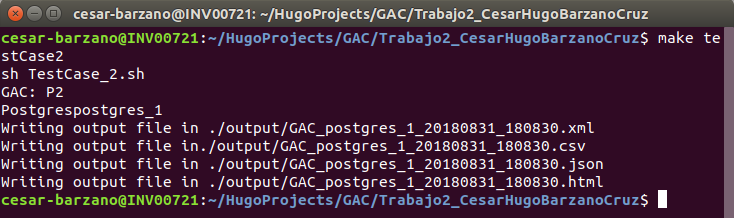
\includegraphics[scale=0.35]{imagenes/TestCase2_1.png}
\caption{ Test Case 2 }  
\end{figure} 




\subsubsection{Test Case 3 - Sqlite3 }

A continuación se muestra la configuración utilizada por el generador para el tercer caso de pruaba. 

\begin{lstlisting}[language=python,caption={GAC\_GENERATOR\_CONFIG\_3.json }]
 {
  "sqlite3_1": {
    "db_path": "./testGAC.db"
  }
}

\end{lstlisting}


El tercer caso de prueba puede ejecutarse mediante make testCase3, el resultado es similitar al caso de prueba 1 y 2. 

\begin{figure}[H]  
\centering 
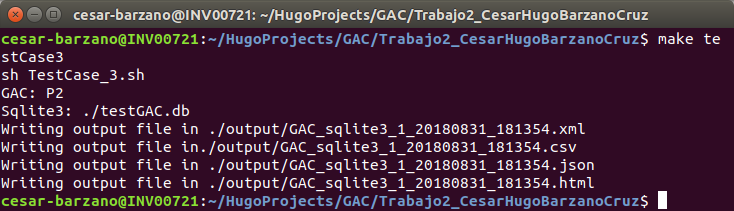
\includegraphics[scale=0.35]{imagenes/TestCase3_1.png}
\caption{ Test Case 3 }  
\end{figure} 


\subsubsection{Test Case 4 - WHERE}

El cuarto caso de prueba muestra el uso de la clausula WHERE para filtrar los resultados del generador. De manera adicional el caso de prueba número 4 trata de mostrar la capacidad del generador para utilizar varios SGBD establecidos en la misma configuración. Por simplicidad se va a utilizar la misma base de datos mysql pero a efectos prácticos de configuración, podrian ser 2 SGBD totalmente independientes. 

\begin{lstlisting}[language=python,caption={GAC\_GENERATOR\_CONFIG\_4.json }]
  {
	"mysql_1": {
		"user": "root",
		"password": "root",
		"host": "localhost",
		"database": "testGAC"
	},
	"mysql_2": {
		"user": "root",
		"password": "root",
		"host": "127.0.0.1",
		"database": "testGAC"
	}
}
\end{lstlisting}

Para mostrar la capacidad de filtrado mediante clausula WHERE, se van a filtrar todos los modelos cuyo número sea 1 es, es decir, --where "model\_no = '1'". El cuarto caso de prueba puede ser ejecutado mediante make testCase4

\begin{figure}[H]  
\centering 
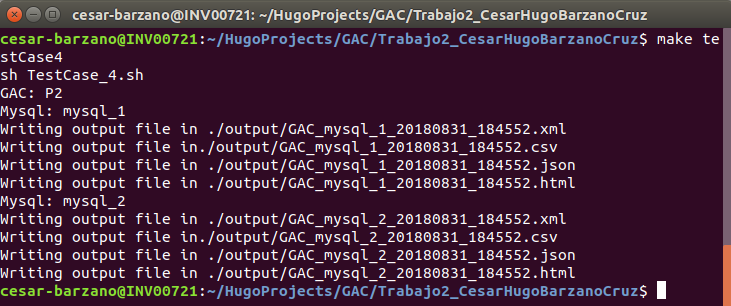
\includegraphics[scale=0.35]{imagenes/TestCase4_1.png}
\caption{ Test Case 3 }  
\end{figure}

La ejecución del cuarto caso de prueba produce las siguientes salidas dentro del directorio output, 4 ficheros con los correspondientes formatos para mysql\_1 junto con otros 4 ficheros con los correspondientes formatos para mysql\_2. Como indicamos anteriormente las bases de datos son similares por lo que a continuación solo se va a mostrar los ficheros generados para mysql\_2. 


\begin{lstlisting}[language=python,caption={Formato CSV }]
1,atribute_1,atribute_2
\end{lstlisting}

\begin{lstlisting}[language=python,caption={Formato HTML }]
<!DOCTYPE html>
    <html>
    <head>
    <title>mysql_2</title>
    </head>
    <body>
    <h1>mysql_2</h1><hr><br><table style="width:100%"><tr><td>1</td><td>atribute_1</td><td>atribute_2</td></tr></table></body></html> 
\end{lstlisting}

El resultado del generador para formato HTML queda mas claro si es interpretado por el navegador: 

\begin{figure}[H]  
\centering 
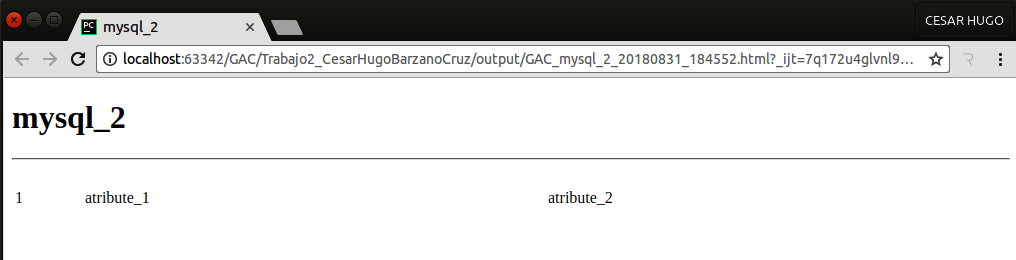
\includegraphics[scale=0.35]{imagenes/TestCase4_html.png}
\caption{ Test Case 4 - HTML Output }  
\end{figure} 


\begin{lstlisting}[language=python,caption={Formato Json }]
[[1, "atribute_1", "atribute_2"]]
\end{lstlisting}


\begin{lstlisting}[language=python,caption={Formato XML }]
<data>&lt;data&gt;&lt;i&gt;&lt;i&gt;1&lt;/i&gt;&lt;i&gt;atribute_1&lt;/i&gt;&lt;i&gt;atribute_2&lt;/i&gt;&lt;/i&gt;&lt;/data&gt;</data>
\end{lstlisting}

El resultado del generador para formato xml queda mas claro si es interpretado por el navegador: 

\begin{figure}[H]  
\centering 
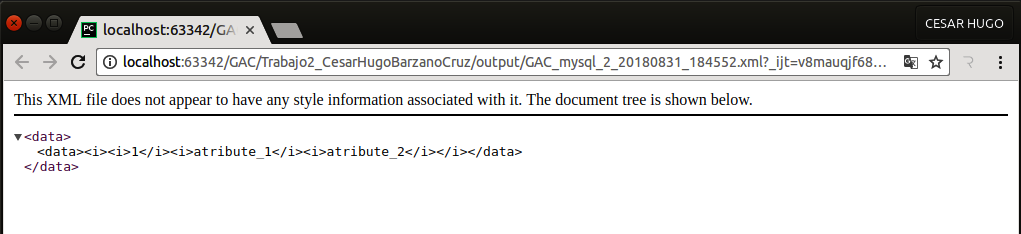
\includegraphics[scale=0.35]{imagenes/TestCase4_xml.png}
\caption{ Test Case 4 - XML Output }  
\end{figure} 

\subsubsection{Test Case 5 - All SGBD}

El quinto caso de prueba muestra la capacidad del generador para producir salida involucrando a todos los SGBD soportados por el mismo. Para ello, a continuación se muestra la configuración aplicada al generador. 

\begin{lstlisting}[language=python,caption={GAC\_GENERATOR\_CONFIG\_5.json }]
 {
	"mysql_1": {
		"user": "root",
		"password": "root",
		"host": "localhost",
		"database": "testGAC"
	},
	"mysql_2": {
		"user": "root",
		"password": "root",
		"host": "127.0.0.1",
		"database": "testGAC"
	},
  "postgres_1": {
		"user": "postgres",
		"password": "123456",
		"host": "127.0.0.1",
		"database": "testgac"
	},
  "sqlite3_1": {
    "db_path": "./testGAC.db"
  }
}
\end{lstlisting}

El quinto caso de prueba puede ser ejecutado mediante  make testCase5 el cual genera en el directorio output 4 ficheros con los correspondientes formatos para cada uno de los SGBDs configurados. 

\begin{figure}[H]  
\centering 
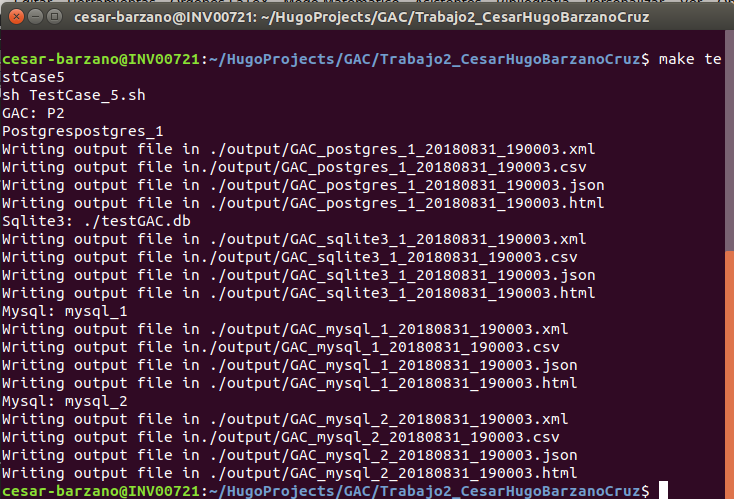
\includegraphics[scale=0.35]{imagenes/TestCase5_1.png}
\caption{ Test Case 5 }  
\end{figure}

No se va a mostrar el contenido de los ficheros generador debido a que el estado de las bases de datos no ha cambiado con respecto a los casos de prueba anteriores. 

 
 


 
\subsection{Pruebas de Error} 

Para realizar las pruebas de error, se han definido 2 escenarios.

\subsubsection{Test Case Error - 1}

En el primer escenario de error, las credenciales para conectar con el SGBD son erroneas. 

\begin{lstlisting}[language=python,caption={GAC\_GENERATOR\_CONFIG\_error.json }]
{
	"mysql_1": {
		"user": "bad_user",
		"password": "bad_pass",
		"host": "localhost",
		"database": "testGAC"
	},
  "postgres_1": {
		"user": "bad_user",
		"password": "bad_pass",
		"host": "127.0.0.1",
		"database": "testgac"
	}
}
\end{lstlisting}

El primer caso de error puede ser ejecutado mediante make testCaseError1. Como podemos observar, el generador continua su ejecución intentando conectarse a los distintos SGBD configurados. 

\begin{figure}[H]  
\centering 
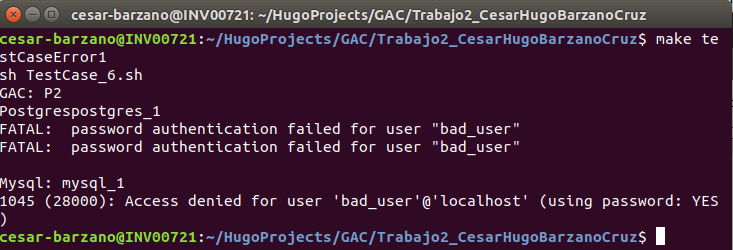
\includegraphics[scale=0.35]{imagenes/TestCase6_1.png}
\caption{ Test Case Error - 1 }  
\end{figure}

\subsubsection{Test Case Error - 2}

Para el segundo escenario de error se va a aplicar la misma configuración y ejecución. La  diferencia esta en que los servicios locales que representas los SGBD configurados estaran detenidos, de esta manera podemos simular que tanto los host como los SGBD no estan disponibles para su conexión. 

Los SGBD usados para este escenario pueden ser detenidos mediante: 
\begin{enumerate}
\item \textbf{mysql: sudo /etc/init.d/mysql stop }
\item \textbf{postgres: sudo service postgresql stop}
\end{enumerate}

\begin{figure}[H]  
\centering 
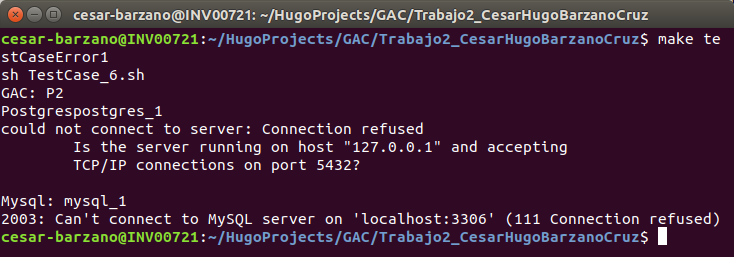
\includegraphics[scale=0.35]{imagenes/TestCase6_2.png}
\caption{ Test Case Error - 2 }  
\end{figure}





\chapter{Entrega}
En este capítulo se detallan cada uno de los ficheros/directorios que forman parte de la entrega. 

\section{Generador}
El generador propuesto por el enunciado se compone de un único fichero denominado generadorP2.py el cual se encuentra alojado en la raíz del fichero comprimido que se envía. El generador ha sido desarrollado sobre Ubuntu18 y hace uso de la versión python 2.7.15. Si alguna de ellas causará error, podría ser instalada fácilmente descargando el paquete de las URLs indicadas en la bibliografía y ejecutando sudo pip install nombre\_paquete 

\section{Makefile}
El fichero ''makefile'' establece las distintas ejecuciones de pruebas para el generador. Tambien dispone de la entrada ''make doc'' para generar la especificación software mediante pydoc. Alojado en la raíz del fichero comprimido para la entrega. 

\section{Directorio software specification}
Contiene la especificación del generador en formato HTML. Dicha especificación ha sido generada utilizando la librería pydoc. 

\section{Trabajo2\_CesarHugoBarzanoCruz.pdf}
Memoría de la práctica, referencia a este documento en si mismo, alojado en el directorio raíz de la entrega. 

\section{Directorio DOC}
Directorio donde se almacenan todos los fuentes usados para generar esta documentación utilizando LaTEX. Incluye tambien las imagenes usadas en la memoria. 

\section{Directorio input}
Directorio donde se almacenan todos los ficheros usados como configuracion para el generador.

\section{Directorio Output}
Directorio donde se almacenan todos los ficheros resultados de la ejecución de la pruebas. 

 

\begin{thebibliography}{aaaa}

%intro

\bibitem[1]{xml} \textsc{XML},
\textit{XML Format}
\url{https://www.w3.org/XML/} 


\bibitem[2]{json} \textsc{JSON},
\textit{JSON Format}
\url{https://www.json.org/} 

%Desarrollo

\bibitem[3]{py} \textsc{python},
\textit{Python 2.7.6 language}
\url{https://www.python.org/download/releases/2.7.6/} 


\bibitem[4]{json_lib} \textsc{import json},
\textit{JSON encoder and decoder}
\url{https://docs.python.org/2/library/json.html} 

\bibitem[5]{xmltodic_lib} \textsc{import xmltodic},
\textit{Makes working with XML feel like you are working with JSON}
\url{https://pypi.python.org/pypi/xmltodict} 

\bibitem[6]{sys_lib} \textsc{import sys},
\textit{System-specific parameters and functions}
\url{https://docs.python.org/2/library/sys.html} 

\bibitem[7]{os_lib} \textsc{import os},
\textit{Miscellaneous operating system interfaces}
\url{https://docs.python.org/2/library/os.html} 

\bibitem[8]{getopt_lib} \textsc{import getopt},
\textit{C-style parser for command line options}
\url{https://docs.python.org/2/library/getopt.html}


\end{thebibliography}
 

\chapter{Anexo}
\section{generator.py}
\begin{lstlisting}[language=python,caption={generatorP2.py }]
#!/usr/bin/python


__author__ = 'Hugo Barzano'
__date__ = '2017/2018'
__version__ = 'v1.0'
__credits__ = 'GAC'
__file__ = 'generatorP2.py'


import sys
import os
import getopt
import time
import mysql.connector
import json
import psycopg2
import sqlite3
import lxml.etree as et
import csv
import io


#INPUT and OUTPUT DATA FOLDER
OUTPUT_FOLDER="./output/"
INPUT_FOLDER="./input/"

"""Generator configuration file: Databases interfaces definition"""
#CONFIG=INPUT_FOLDER+"GENERATOR_CONFIG.json"
CONFIG=os.environ['GENERATOR_CONFIG']
def data2xml(data, name='data'):
    root = et.Element(name)
    return et.tostring(buildxml(root, data))

def buildxml(root, data):
    if isinstance(data, dict):
        for key, value in data.iteritems():
            sub = et.SubElement(root, key)
            buildxml(sub, value)
    elif isinstance(data, tuple) or isinstance(data, list):
        for value in data:
            sub = et.SubElement(root, 'i')
            buildxml(sub, value)
    elif isinstance(data, basestring):
        root.text = data
    else:
        root.text = str(data)
    return root

def buildCsv(data,sgbd):
    with open(OUTPUT_FOLDER+"GAC_"+sgbd+"_"+time.strftime("%Y%m%d_%H%M%S")+".csv", "w") as output:
        writer = csv.writer(output, lineterminator='\n')
        writer.writerows(data)
    print "Writing output file in"+OUTPUT_FOLDER+"GAC_"+sgbd+"_"+time.strftime("%Y%m%d_%H%M%S")+".csv"

def buildHtml(data,sgbd):
    html_table_1="""<table style="width:100%">"""
    html_table_2=""
    for tupla in data:
        html_table_2="<tr>"
        for t in tupla:
            html_table_2=html_table_2+"<td>"+str(t)+"</td>"
        html_table_2=html_table_2+"</tr>"
    html_table=html_table_1+html_table_2+"</table>"
    html_doc="""<!DOCTYPE html>
    <html>
    <head>
    <title>"""+sgbd+"""</title>
    </head>
    <body>
    <h1>"""+sgbd+"""</h1><hr><br>"""+html_table+"""</body></html> """
    return html_doc

def writeOutput(output_file,output_string):
    """Function to write output files.
         :param output_file: output file path
         :param output_string: string to write in the output file"""
    print "Writing output file in "+output_file
    try:
        with open(output_file, 'w') as f:
    	       f.write(output_string)
    except EnvironmentError:
        print("Oops! Error writing output file...")
        exit()

def configurePostgres(config_json):
    config_str="host='"+config_json["host"]+"' dbname='"+config_json["database"]+"' user='"+config_json["user"]+"' password='"+config_json["password"]+"'"
    return config_str

def main(argv):
    #python generadorP2.py -t gac_models -w "atr_1 = 'atribute_1'"
    """Main method to execute the generator.
                :param argv: value from 0 to n-1 to ident"""
    table=None
    where=None
    debug=False

    # process arguments
    try:
        opts, args = getopt.getopt(argv, "hvt:w:d", ["help", "version", "table=","where=","debug"])
    except getopt.GetoptError as err:
        print str(err)
        usage()
        sys.exit(2)
    for opt, arg in opts:
        if opt in ("-h", "--help"):
            usage()
            sys.exit()
        elif opt in ("-v", "--version"):
            version()
            sys.exit()
        elif opt in ("-t", "--table"):
            table = arg
        elif opt in ("-w","--where"):
            where=arg
        elif opt in ("-d", "--debug"):
            debug = True
            print "Debug: TRUE"
        else:
            usage()
            sys.exit()

    print "GAC: P2"
    with open(CONFIG) as config_file:
        SGBD_config = json.load(config_file)

    if where==None:
        query = ("SELECT * FROM "+table)
    else:
        query = ("SELECT * FROM "+table+ " WHERE "+where)
    connector=None
    cursor=None
    data=None
    for SGBD in SGBD_config:
        if "mysql" in SGBD:
            print "Mysql: "+ SGBD
            try:
                connector = mysql.connector.connect(**SGBD_config[SGBD])
            except mysql.connector.Error as err:
                print(err)
                continue
        elif "postgres" in SGBD:
            print "Postgres"+ SGBD
            try:
                connector = psycopg2.connect(configurePostgres(SGBD_config[SGBD]))
            except psycopg2.OperationalError as err:
                print (err)
                continue
        elif "sqlite3" in SGBD:
            print "Sqlite3: "+SGBD_config[SGBD]["db_path"]
            try:
                connector=sqlite3.connect(SGBD_config[SGBD]["db_path"])
            except Exception as err:
                print "no sql3"
                print (err)
                continue
        else:
            print SGBD+" Not SGBD supported"

        cursor = connector.cursor()
        cursor.execute(query)
        data=cursor.fetchall()
        if data != None:
            """XML FILE"""
            xml_data=data2xml(data2xml(data, name='data'))
            writeOutput(OUTPUT_FOLDER+"GAC_"+SGBD+"_"+time.strftime("%Y%m%d_%H%M%S")+".xml",xml_data)

            """CSV FILE"""
            buildCsv(data,SGBD)

            """HTML FILE"""
            jsonObj = json.dumps(data)
            writeOutput(OUTPUT_FOLDER+"GAC_"+SGBD+"_"+time.strftime("%Y%m%d_%H%M%S")+".json",jsonObj)

            """HTML FILE"""
            html_doc=buildHtml(data,SGBD)
            writeOutput(OUTPUT_FOLDER+"GAC_"+SGBD+"_"+time.strftime("%Y%m%d_%H%M%S")+".html",html_doc)
        else:
            print "No data"
    #isinstance(object, classinfo)


# --------------------------------------------------------------------------------------------------
# Main exec
# --------------------------------------------------------------------------------------------------

def usage():
    """Method to display generator usage. """
    print """
Usage: python generador.py [options]

Options
-v, --version			Show the version of this script
-h, --help			Show this help.
-t <table_name>, --table <table_name>   Input database table
-w <"column = 'value'">, --where <"column = 'value'">   Optional Where Clause
-d,         --debug         	Debug Mode
"""

def version():
    """Function to display software version"""
    print "version 1.0"

if __name__ == "__main__":
    if len(sys.argv) > 1:
        main(sys.argv[1:])
    else:
        usage()
        sys.exit()

\end{lstlisting}

\section{makefile}
\begin{lstlisting}[language=python,caption={makefile }]


\end{lstlisting}



%
%
%%\nocite{*}
%\bibliography{bibliografia/bibliografia}\addcontentsline{toc}{chapter}{Bibliografía}
%\bibliographystyle{miunsrturl}
%
%\appendix

%\input{apendices/manual_usuario/manual_usuario}
%%\input{apendices/paper/paper}
%\input{glosario/entradas_glosario}
% \addcontentsline{toc}{chapter}{Glosario}
% \printglossary

\thispagestyle{empty}

\end{document}
